% !TEX TS-program = PDFLatexBibtex
%&LaTeX
\documentclass[]{elsarticle}
\setlength{\marginparwidth}{0.5in}
\usepackage{amsmath,amssymb,amsthm,natbib,
mathtools,bbm,extraipa,mathabx,graphicx,algorithm}
\usepackage{algpseudocode}
%accents,

\newtheorem{lem}{Lemma}
\newtheorem{remark}{Remark}
\newtheorem{theorem}{Theorem}
\newtheorem{definition}{Definition}
\newtheorem{proposition}{Proposition}
\theoremstyle{definition}
\newtheorem{algo}{Algorithm}

\newcommand{\fudge}{\fC}
\newcommand{\dtf}{\textit{\doubletilde{f}}}
\newcommand{\cube}{[0,1)^d}
%\renewcommand{\bbK}{\natzero^d}
\newcommand{\rf}{\mathring{f}}
\newcommand{\rnu}{\mathring{\nu}}
\newcommand{\natm}{\naturals_{0,m}}
\newcommand{\wcS}{\widecheck{S}}
\newcommand{\tol}{\text{tol}}
\newcommand{\e}{\text{e}}
\newcommand{\bvec}[1]{\boldsymbol{#1}}
\newcommand{\vx}{\bvec{x}}
\newcommand{\vI}{\bvec{I}}
\newcommand{\vk}{\bvec{k}}
\newcommand{\vw}{\bvec{w}}
\newcommand{\vz}{\bvec{z}}
\newcommand{\dif}{\mathsf{d}}
\newcommand{\hf}{\hat{f}}
\newcommand{\hS}{\widehat{S}}
\newcommand{\tS}{\widetilde{S}}
\newcommand{\tf}{\tilde{f}}
\newcommand{\fC}{\mathfrak{C}}
\newcommand{\homega}{\widehat{\omega}}
\newcommand{\wcomega}{\mathring{\omega}}
\newcommand{\vzero}{\bvec{0}}
\newcommand{\integers}{\mathbb{Z}}
\newcommand{\naturals}{\mathbb{N}}
\newcommand{\ip}[3][{}]{\ensuremath{\left \langle #2, #3 \right \rangle_{#1}}}
\newcommand\iid{\stackrel{iid}{\sim}}

\makeatletter
\newcommand*{\ov}[1]{
  \m@th\overline{\mbox{#1}\raisebox{2mm}{}}
}

\def\abs#1{\ensuremath{\left \lvert #1 \right \rvert}}

\let\oldemptyset\emptyset
\let\emptyset\varnothing


\begin{document}

\begin{frontmatter}

\title{Reliable error estimation for Sobol' indices}

\author{Cl\'ementine Prieur, Elise Arnaud, Laurent Gilquin, Fred J. Hickernell, Llu\'{i}s Antoni Jim\'{e}nez Rugama}
\address{U. Josef Fourier, Illinois Institute of Technology}
\begin{abstract}
\end{abstract}

\end{frontmatter}

\section{Introduction}

\begin{itemize}
\item[$\bullet$] introduction sensitivity analysis + estimation methods
\item[$\bullet$] importance of sampling $\rightarrow$ sobol' sequences
\item[$\bullet$] problem: when to stop? $\rightarrow$ reliable error estimation 
\end{itemize}

\section{Backgrounds on Sobol' indices}

\subsection{Definition of Sobol' indices}
%We adopt the same notations introduced by Owen in \cite{Owen}. 
Denote by $f$ a numerical model, by $\vx=(x_1,\dots,x_d)$ its vector of inputs and set $\mathcal{D}=\{1,\dots,d\}$. The uncertainty on $\vx$ is modeled by a random vector that we suppose uniformly distributed on $\cube$. Let $u$ be a subset of $\mathcal{D}$, $-u$ its complement and $|u|$ its cardinality. $\vx_u$ represents a point in $[0,1)^u$ with components $x_j, j \in u$. Given two points $\vx$ and $\vx'$, the hybrid point $\vw=(\vx_u:{\vx'}_{-u})$ is defined as $w_j=x_j$ if $j \in u$ and $w_j={x'}_j$ if $j \notin u$.

Let $f$ be the symbol representing the numerical model studied. We assume $f \in \mathcal{L}^2[0,1)^d$. Denote by $\mu$ and $\sigma^2$ the mean and variance of $f$.
The uncertainty on $\vx$ is modeled by random variables such that $\vx \iid \mathcal{U}[0,1)^d$. Recall the Hoeffding decomposition \cite{Hoeffding} of $f$:
\begin{equation}
f(\vx)=\mu+\sum \limits_{u \subseteq \mathcal{D}} f_u(\vx),
\label{anova}
\end{equation}
where:
\[f_u(\vx)= \int_{[0,1)^{|u|}} f(\vx) d{\vx}_{-u} - \sum \limits_{v \subset u} f_v(\vx).\]
Due to orthogonality, taking the variance of each side in equation (\ref{anova}) leads to the variance decomposition of $f$:
\[ \sigma^2 = \sum \limits_{u \subseteq \{1,\dots,d\}} \sigma_v^2, \ \text{ with } \ \sigma_v^2=\int_{[0,1)^{|v|}} f_v(\vx)^2 d{\vx}.\]
From the variance decomposition of $f$, on can express the following two quantities:
\[\underline{\tau}_u^2 = \sum \limits_{v \subseteq u} \sigma_v^2, \qquad
\ov{$\tau$}_u^2 = \sum \limits_{v \cap u \neq \varnothing} \sigma_v^2, \qquad u \subsetneq \mathcal{D}.\]

For $u \subsetneq \mathcal{D}$, the two quantities $\underline{\tau}_u^2$ and $\ov{$\tau$}_u^2$ both measure the importance of the variables in $\vx_u$. $\underline{\tau}_u^2$ quantifies the main effect of $\vx_u$ that is the effect of all interactions between variables in $\vx_u$. $\ov{$\tau$}_u^2$ quantifies the main effect of $\vx_u$ plus all interactions between variables in $\vx_u$ and variables in $\vx_{-u}$.

$\underline{\tau}_u^2$ and $\ov{$\tau$}_u^2$ satisfy the following relations: $ 0 \leq  \underline{\tau}_u^2 \leq \ov{$\tau$}_u^2$ and $\underline{\tau}_u^2 = \sigma^2 - \ov{$\tau$}_{-u}^2$. These two measure are commonly found in the litterature in their normalized form: $\underline{S}_u = \underline{\tau}_u^2 / \sigma^2$ is the closed $|u|$-order Sobol' index for the set $u$, while $\ov{$S$}_u = \ov{$\tau$}_u^2 / \sigma^2$ is the total effect Sobol' index for the set $u$.
\bigskip

The problem of interest here is the evaluation of first-order and total effect Sobol' indices. The computation of these indices is performed based on the following integral formula for their numerators:
\begin{align}
\label{first.order}
\underline{\tau}_u^2  &= \int_{[0,1)^{2d-1}} \left(f(\vx)-
f(\vx_u:{\vx'}_{-u})\right)f(\vx')d\vx d{\vx'}, \\
\label{total.effect}
\ov{$\tau$}_u^2 &= \frac{1}{2}\int_{[0,1)^{d+1}}(f(\vx')-f(\vx_u:{\vx'}_{-u}))^2d\vx d{\vx'}, \qquad u \in \mathcal{D},
\end{align}
The variance of $f$ is evaluated by:
\[ \sigma^2 = \int_{[0,1)^{d}} f(\vx)^2d{\vx} - \mu^2, \text{ with } \ \mu = \int_{[0,1)^{d}} f(\vx) d{\vx}.\]
Most of the time, the complexity of $f$ causes the computation of $\mu$, $\sigma^2$ and integrals (\ref{first.order}) and (\ref{total.effect}) to be intractable. In such case, one needs to rely on an estimation of these quantities.

\subsection{Estimation of Sobol' indices}
\label{estimation.strategies}
In this section we review two Monte Carlo procedures for the estimation of Sobol' indices. We define by design a point set $\mathcal{P}=\{\vx_i\}_{i=0}^{n-1}$ obtained by sampling each variable $x_j$ $n$ times. Each row of the design is a point $\vx_i$ in $[0,1)^d$. Each column of the design refers to a variable $x_j$. Consider $\mathcal{P}=\{\vx_i\}_{i=0}^{n-1}$ and $\mathcal{P'}=\{{\vx'}_i\}_{i=0}^{n-1}$ two designs where $(\vx_i,{\vx'}_i) \iid [0,1)^{2d}$. 
\bigskip

One way to estimate the two quantities (\ref{first.order}) and (\ref{total.effect}) is via:
\begin{align}
\label{first.order.est}
\widehat{\underline{\tau}_u^2} & = \frac{1}{n} \sum \limits_{i=0}^{n-1} \left(f(\vx_i)-f(\vx_{i,u}:{\vx'}_{i,-u}\right)f(\vx'_i),\\
\label{total.effect.est}
\widehat{\ov{$\tau$}_u^2} & = \frac{1}{2n} \sum \limits_{i=0}^{n-1} (f({\vx'}_i) - f(\vx_{i,u}:{\vx'}_{i,-u}))^2, \qquad u \in \mathcal{D},
\end{align}
using for $\sigma^2$ the classic estimator:
\begin{equation}
 \widehat{\sigma}^2 = \frac{1}{n} \sum \limits_{i=0}^{n-1} f(\vx_i)^2 - \widehat{\mu}^2, \text{ with } \ \widehat{\mu} =  \frac{1}{n} \sum \limits_{i=0}^{n-1} f(\vx_i).
\label{mu.est}
\end{equation}
The estimation of a single pair ($\underline{\tau}_u^2$, $\ov{$\tau$}_u^2$) requires $3n$ evaluations of the model $f$. Using a combinatorial formalism, in \cite[Theorem 1]{Saltelli} Saltelli proposes the following estimation strategy:
\begin{theorem}
\label{saltelli.theorem}
The $d+2$ designs $\{\vx_{i,u},{\vx'}_{i,-u}\}_{i=0}^{n-1}$ constructed for $u \in \{\varnothing,\{1\},\dots,$ $\{d\},\mathcal{D}\}$ allows to estimate all first-order and all total effect Sobol' indices at a cost of $n(d+2)$ evaluations of the model.
\end{theorem}
The $d+2$ designs of Theorem \ref{saltelli.theorem} are obtained by substituting columns of $\mathcal{P}$ for columns of $\mathcal{P}'$ accordingly to $u$. While elegant, this approach still requires a number of model evaluations that grows linearly with respect to the input space dimension.

An efficient alternative to evaluate all first-order indices was proposed by Mara \textit{et al.} \cite{Mara}  requiring only $2n$ model evaluations. This alternative relies on the construction of two replicated designs. The notion of replicated designs was first introduced by McKay through its introduction of replicated Latin Hypercubes in \cite{Mckay}. The definition we give here introduce the structure in a wider context:
\begin{definition}
\label{rep.designs}
Let $\mathcal{P}=\{\vx_i\}_{i=0}^{n-1}$ and $\mathcal{P}'=\{{\vx'}_i\}_{i=0}^{n-1}$ be two point sets in
$[0,1)^{d}$. Let $\mathcal{P}^u=\{\vx_{i,u}\}_{i=0}^{n-1}$ (resp. ${\mathcal{P}'}^u$), $u \subsetneq \mathcal{D}$, denote the subset of dimensions of $\mathcal{P}$ (resp. $\mathcal{P}'$) indexed by $u$. We say that $\mathcal{P}$ and $\mathcal{P}'$ are two replicated designs of order $a \in \{1,\dots,d-1\}$ if $\forall \ u \subsetneq \mathcal{D}$ of cardinality $|u|=a$, $\mathcal{P}^u$ and ${\mathcal{P}'}^u$ are the same point set in $[0,1)^a$. We note $\pi_u$ the permutation reordering the rows of ${\mathcal{P}'}^u$ into $\mathcal{P}^u$.
\end{definition}
The method introduced in \cite{Mara} allows to estimate all first-order Sobol' indices with only two replicated designs of order $1$. The key point of this method is to use the permutations resulting from the structure of the two replicated designs to mimic the hybrid points in formula (\ref{first.order.est}). 

More specifically, let $\mathcal{P}=\{\vx_i\}_{i=0}^{n-1}$ and $\mathcal{P}'=\{{\vx'}_i\}_{i=0}^{n-1}$ be two replicated designs of order $1$. Denote by $\{f(\vx_i)\}_{i=0}^{n-1}$ and $\{f({\vx'}_i)\}_{i=0}^{n-1}$ the two sets of model evaluations obtained with $\mathcal{P}$ and $\mathcal{P}'$. Consider $u \in \mathcal{D}$, from Definition \ref{rep.designs} there exists a permutation $\pi_u$ such that ${\vx'}_{\pi_u(i),u}={\vx}_{i,u}$. Then, remark that $\forall i \in \{0,\dots,n-1\}$:
\[\pi_u(f({\vx'}_i))=f({\vx'}_{\pi_u(i)})=f(\vx'_{\pi_u(i),u}:{\vx'}_{\pi_u(i),-u})=f(\vx_{i,u}:{\vx'}_{\pi_u(i),-u})\]
%\pi_u(f({\vx'}_{i,u}:{\vx'}_{i,-u}))
Each $\underline{\tau}^2_u$ can be estimated via formula (\ref{first.order.est}) with $\{f(\vx_i)\}_{i=0}^{n-1}$ and $\{\pi_u(f({\vx'}_i))\}_{i=0}^{n-1}$ without requiring further model evaluations. This estimation method has been deeply studied and generalized in Tissot et al. \cite{Mara} to the case of closed second-order indices. In the following we refer to this method as replication procedure.
\bigskip

\subsection{Towards a reliable estimation}
The aim of this paper is to propose a recursive estimation procedure to estimate Sobol' indices. The choice of the stopping criterion is the key point of this paper. 

The two estimation procedures reviewed in the previous section can be rendered recursive. In \cite{Gilquin16}, the authors propose a recursive version of the replication procedure. In this recursive version, the stopping criterion is an absolute difference between estimates computed on consecutive steps. More generally, in most recursive approaches that estimate Sobol' indices, the stopping criterion is a quantity of interest build directly upon the estimates. Such stopping criteria often involved hyperparameters hard to tweak but above all fail to guarantee any error bound on the estimation. 
\bigskip

Our recursive procedure stands apart from others approaches by the construction of a robust stopping criterion. This criterion is an error bound based on the discrete Walsh decomposition of integrals (\ref{first.order}) and (\ref{total.effect}). This decomposition use the close set property of digital sequences. As such, our recursive procedure relies on the iterative construction of Sobol' sequences. The iterative construction of the Sobol' sequences is performed accordingly to the multiplicative  approach presented in \cite{crass}.

The construction of our stopping criterion is the subject of the next section \ref{section.error}. Our recursive estimation procedure is presented in section \ref{section.recursive.procedure}.


\section{Reliable Error Estimation for Cubatures}
\label{section.error} 

\subsection{Reliable Estimation Using Quasi-Monte Carlo}\label{sec_reliable_error}


Consider an embedded sequence of digital nets in base $b$,
\[
\mathcal{P}_0=\{\bvec{0}\}\subset\dots\subset\mathcal{P}_m=\{\vx_i\}_{i=0}^{b^m-1}\subset\dots\subset\mathcal{P}_\infty=\{\vx_i\}_{i=0}^{\infty}.
\]
One example that will be particularly useful for our application is the Sobol' sequence \cite{•}.

Each $\mathcal{P}_m$ has a group structure under the digit wise addition. Analogously, we can also define the dual nets as $\mathcal{P}_m^\perp=\{\vk\in\mathbb{N}_0^d:\ip{\vx}{\vk}=0,\, \vx\in\mathcal{P}_m\}$,
\[
\mathcal{P}_0^\perp=\left\{\mathbb{N}_0^d\right\}\supset\dots\supset\mathcal{P}_\infty=\{\bvec{0}\}.
\]

An important property for the error estimation using digital nets is that for any Walsh basis $\phi_{\vk}(\vx)$
\begin{equation}\label{basis_prop}
\frac{1}{b^m}\sum_{\vx\in\mathcal{P}_m}\phi_{\vk}(\vx)=
\begin{cases}
1,\quad \vk\in\mathcal{P}_m^\perp, \\
0,\quad \vk\notin\mathcal{P}_m^\perp.
\end{cases}
\end{equation}

For any function $f\in L^2(\cube)$, one may use its Walsh series $f(\vx)=\sum_{\vk\in\naturals_0^d}\hf_{\vk}\phi_{\vk}(\vx)$ and equation \eqref{basis_prop} to rewrite the error as,


\[
\abs{\int_{\cube} f(\vx)\,d\vx - \frac{1}{b^m}\sum_{\vx\in\mathcal{P}_m}f(\vx)}=\abs{\sum_{\vk\in\mathcal{P}_m^\perp\setminus\{\vzero\}}\hf_{\vk}}
\]

In \cite{HicJim} we proposed an algorithm based on digital nets that estimates hight dimensional integrals whose error lies within a user-input error tolerance. This algorithm finds the number of data points automatically. We will refer to it as $\widehat{I}(f;\varepsilon)$, where $f$ is the function to integrate and $\varepsilon$ the user-input error tolerance.

The main result from the article if that for all $f\in\mathcal{C}$,
\[
\abs{\int_{\cube} f(\vx)\,d\vx - \widehat{I}(f;\varepsilon)}\leq a(r,m)\sum_{\kappa=\left \lfloor 2^{m-r-1}\right \rfloor}^{2^{m-r}-1} \abs{\tf_{m,\kappa}}\leq \varepsilon.
\]
\begin{itemize}
\item $\tf_{m,\kappa}=$ discrete Fourier Walsh coefficients of $f$.
\item $a(r,m)=$ inflation factor that depends on $\mathcal{C}$.
\end{itemize}

\subsection{Definition of $\widehat{S}$ (fix it with max and min)}

The aim of our algorithm is to estimate the normalized Sobol' indices, $\underline{S}_u = \underline{\tau}_u^2/\sigma^2$ and $\overline{S}_u = \overline{\tau}_u^2/\sigma^2$. In both cases, regular and normalized indices can be approximated by estimating integrals,
\begin{align}\label{indices_integ_1}
\underline{S}_u & = \frac{\int_{[0,1)^{2d-1}} f(\vx)f(\vx_{u}:{\vx'}_{-u})d\vx d{\vx'} - \mu^2 }{\int_{[0,1)^{d}} f(\vx)^2 d{\vx}-\mu^2} = \frac{I_1-(I_3)^2}{I_2-(I_3)^2}, \\
\label{indices_integ_2}
\overline{S}_u & = \frac{\frac{1}{2}\int_{[0,1)^{d+1}}(f(\vx')-f(\vx_u:{\vx'}_{-u}))^2d\vx d{\vx'}}{\int_{[0,1)^{d}} f(\vx)^2 d{\vx}-\mu^2} = \frac{I_1}{I_2-(I_3)^2}.
\end{align}
However, to guarantee the error in our $\underline{S}_u$ and $\overline{S}_u$ approximations we need to proceed with an estimator different than the usual. Given equations \eqref{indices_integ_1} and \eqref{indices_integ_2}, one may write $\underline{S}_u(\vI)$ and $\overline{S}_u(\vI)$ as functions over a vector of integrals $\vI$. According to section \ref{sec_reliable_error}, integrals can be estimated such that $\vI\in B_{\varepsilon_{\vI}}(\widehat{\vI}):=[\widehat{\vI}-\varepsilon_{\vI},\widehat{\vI}+\varepsilon_{\vI} ]$. Thus, the following estimator
\begin{align*}
\widehat{S}_u & = \frac{1}{2}\left(\min\left(\max_{\vI\in B_{\varepsilon_{\vI}}(\widehat{\vI})} S_u(\vI),1\right) + \max\left(\min_{\vI\in B_{\varepsilon_{\vI}}(\widehat{\vI})} S_u(\vI),0\right) \right) \\
\varepsilon_{S_u} & = \frac{1}{2}\left(\min\left(\max_{\vI\in B_{\varepsilon_{\vI}}(\widehat{\vI})} S_u(\vI),1\right) - \max\left(\min_{\vI\in B_{\varepsilon_{\vI}}(\widehat{\vI})} S_u(\vI),0\right) \right)
\end{align*}
ensures that the true value $S_u\in [\widehat{S}_u - \varepsilon_{S_u}, \widehat{S}_u + \varepsilon_{S_u}]$.

\begin{figure}\centering
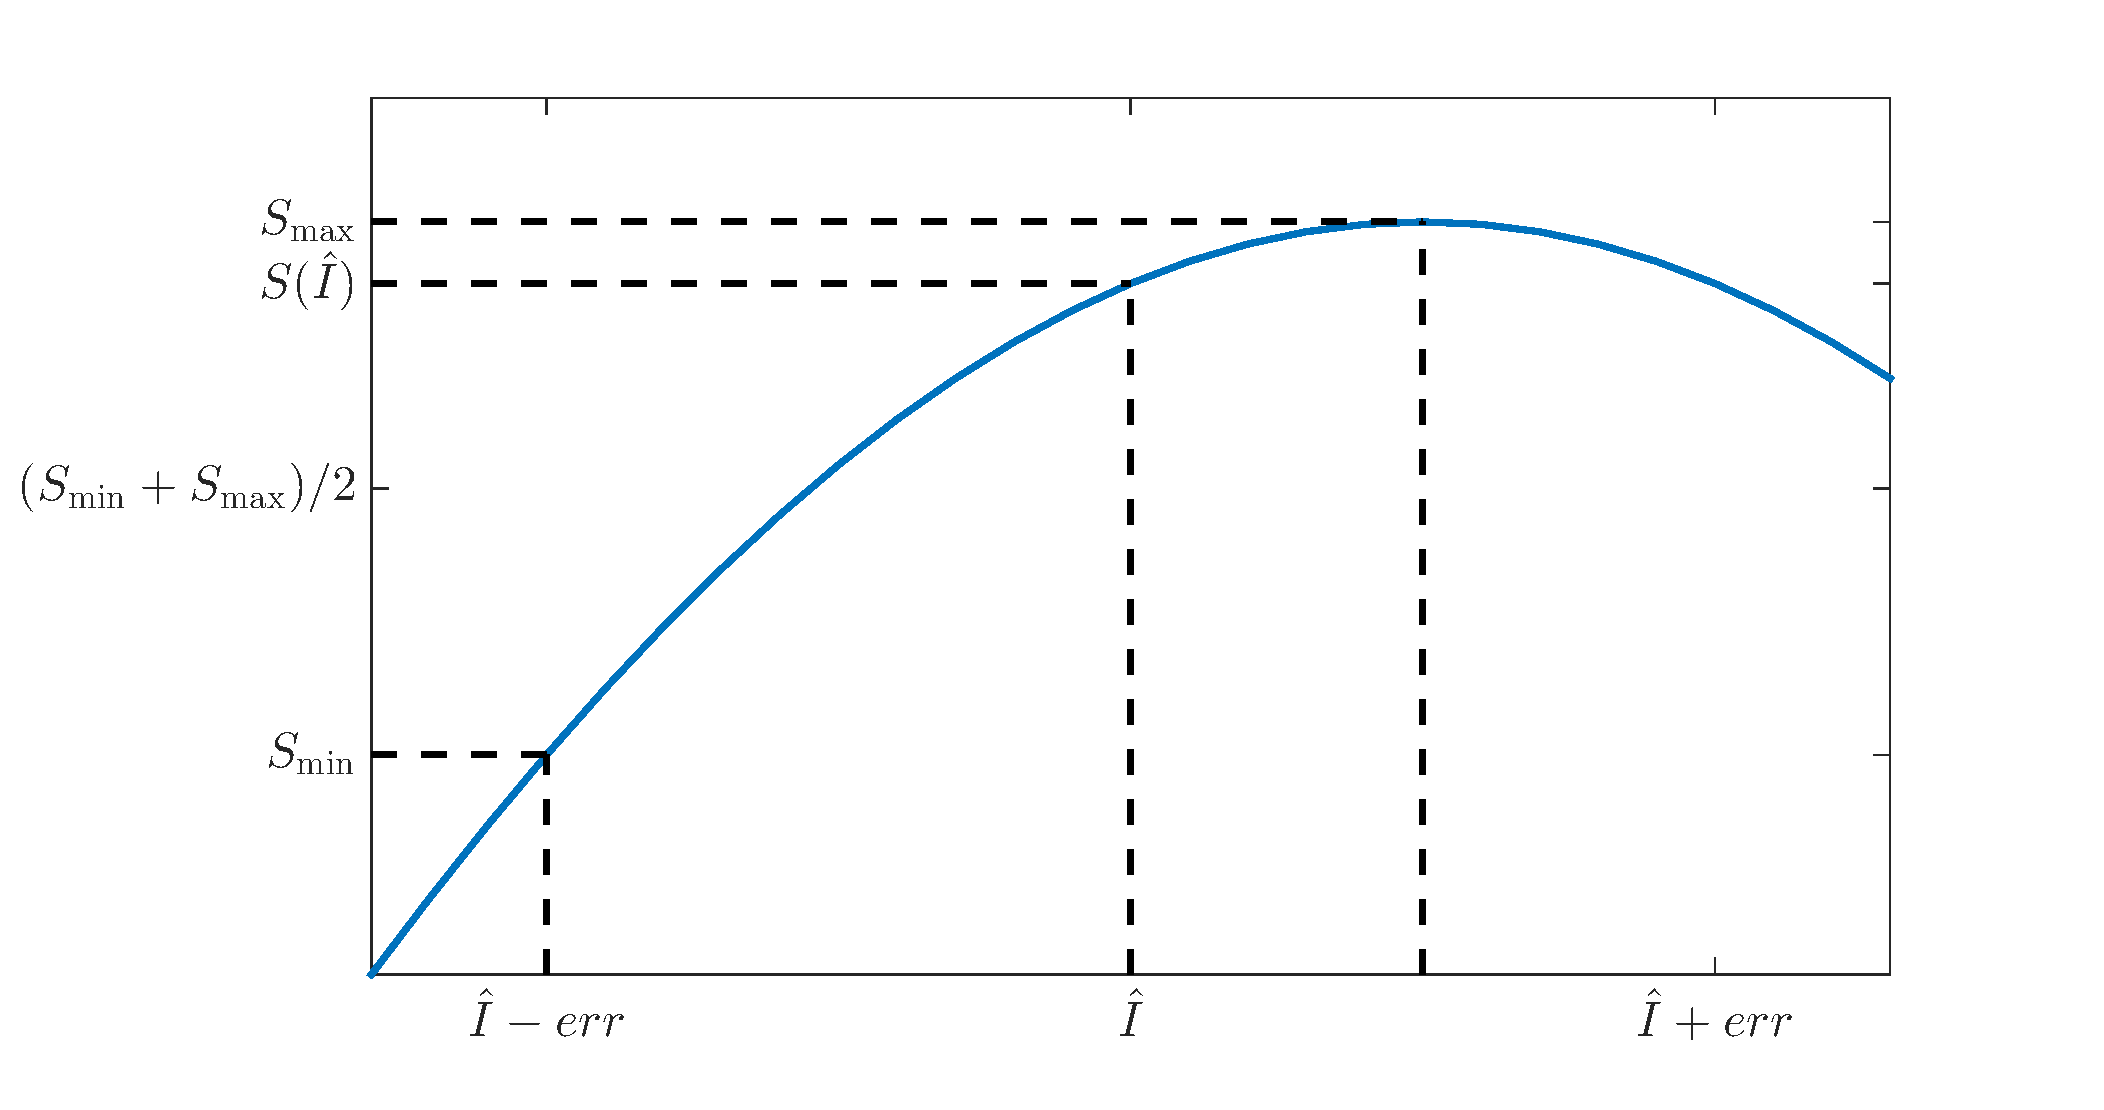
\includegraphics[width=1.\textwidth]{Images/scheme_S.eps}
%\caption*{Representation of estimators.}
\end{figure}

\section{Recursive estimation procedure}
\label{section.recursive.procedure}

The recursive estimation procedure we propose combine the error bound presented in the previous section with one of the two estimation strategies of section \ref{estimation.strategies}. Namely, Saltelli's strategy and the one based on replicated designs. The form of the stopping criterion is the same for both strategies. It is defined as $\abs{\varepsilon_{S_u}} \leq \epsilon$, where $\epsilon$ is the desired precision on the Sobol' indices.

We start be detailing our recursive procedure in the form of an algorithm. Then, we discuss a possible improvement by considering a new estimator recently introduced in \cite{Owen} for first-order indices.

\subsection{Recursive procedure algorithm}

Algorithm \ref{recursive.algorithm} summarizes the main steps of our recursive procedure. First, choose the target tolerance $\epsilon >0$. Choose $r \in \mathbb{N}$ large enough to satisfy the cone conditions (\ref{}) and balance the inflation factor $a(r,\ell)$. Set $\ell=r-1$ and construct the two starting designs $\mathcal{P}_{\ell}=\{\vx_i\}_{i=0}^{2^\ell-1}$ and $\mathcal{P}'_{\ell}=\{\vx'_i\}_{i=0}^{2^\ell-1}$ accordingly to the multiplicative approach detailed in \cite{crass}.

With this construction, at each step $\ell$, $\mathcal{P}_{\ell}$ and $\mathcal{P}'_{\ell}$ correspond to the first $2^\ell$ points of two Sobol' sequences. Furthermore, they possess the structure of two replicated designs of order $1$.
\bigskip

Then, $\mathcal{P}_{\ell}$ and $\mathcal{P}'_{\ell}$ can either be used with Saltelli's strategy to estimate all first-order indices and total effect Sobol' indices. This option is referred as Variant $A$ in Algorithm \ref{recursive.algorithm}. Or $\mathcal{P}_{\ell}$ and $\mathcal{P}'_{\ell}$ can be used with the replication procedure to estimate all first-order Sobol' indices. This option is referred as Variant $B$ in Algorithm \ref{recursive.algorithm}.

If the stopping criterion is satisfied, the algorithm stops and Sobol' estimates are returned. Otherwise, $\ell$ is incremented by one and a new set of $2^{\ell}$ points is added to each design $\mathcal{P}_{\ell}$ and $\mathcal{P}'_{\ell}$. 

\begin{algorithm}[!ht]
\caption{Recursive estimation of Sobol' indices}
\begin{algorithmic}[1]
\vspace*{0.2cm}
\State Choose $\epsilon >0$ and $r \in \mathbb{N}$
\State Set: $\ell \leftarrow r-1$, 
\While {$\abs{\varepsilon_{S_u}} \leq \epsilon$}
\State $\mathcal{P}_\ell \leftarrow \mathcal{P}_{\ell-1} \cup B_\ell$

\hspace*{-0.3cm} $\mathcal{P}'_\ell \leftarrow \mathcal{P}'_{\ell-1} \cup {B'}_\ell$
\For {$u \in \{\varnothing,\{1\},\dots,$ $\{d\},\mathcal{D}\}$}
\If {Variant $A$}
\State Estimate $\widehat{\underline{S}_u}^{(\ell)}$ and $\widehat{\ov{$S$}_u}^{(\ell)}$ with formula \ref{} and Saltelli's strategy
\EndIf
\If {Variant $B$}
\State Estimate $\widehat{\underline{S}_u}^{(\ell)}$ with formula \ref{} and the replication procedure
\EndIf
\EndFor
\State $\ell \leftarrow \ell + 1$
\EndWhile
\State Return the Sobol' estimates.
\end{algorithmic}
\label{recursive.algorithm}
\end{algorithm}

The cost of our algorithm varies whether Variant $A$ or Variant $B$ is selected. To discuss this cost we note by $\ell^\star$ the ending iteration. If Variant $A$ is selected the cost of our algorithm writes:
\begin{equation*}
\sum \limits_{j \in \mathcal{D}} 2^{\ell_j} + 2 \times 2^{\ell^{\star}},
\end{equation*}
where: 
\begin{itemize}
\item[$\bullet$] $2^{\ell_j}$ is the number of evaluations $f\left(\vx_{i,j}:{\vx'}_{i,-j}\right)$ used to estimate both $\underline{S}_j$ and $\overline{S}_j$.
\item[$\bullet$] $2 \times 2^{\ell^{\star}}$ is the number of evaluations $f\left(\vx_{i}\right)$ and $f\left({\vx'}_{i}\right)$ used in the estimation of each first-order and total effect index.
\end{itemize}
This cost can be seen as a generalisation of the one specified in Theorem \ref{saltelli.theorem}. If all $\ell_j$ are equal, the cost of Variant $A$ becomes $2^{\ell^\star}(d+2)$ and we recover the cost of Theorem \ref{saltelli.theorem} with $n=2^{\ell^\star}$.

If Variant $B$ is selected the cost of our algorithm equals $2 \times 2^{\ell^{\star}}$. This cost corresponds to the one specified in the replication procedure with $n=2^{\ell^{\star}}$.

\subsection{Improvements}

We focus on the use of a better estimator to evaluate small first-order Sobol' indices in Variant $A$. This estimator is called ``Correlation 2" and was introduced by Owen in \cite{Owen}. Owen discussed and highlighted the efficiency of ``Correlation 2" when estimating small closed Sobol' indices. Our aim is to show that using ``Correlation 2" in procedure $A$ may reduce the total number of model evaluations. Its formula writes as follows:
\begin{equation}
\widehat{\underline{\tau}_u^2} = \frac{1}{n} \sum \limits_{i=0}^{n-1} (f(\vx_i)-f({\vz}_{i,u}:{\vx}_{i,-u}))(f(\vx_{i,u}:{\vx'}_{i,-u})-f({\vx'}_i)),
\label{correlation2}
\end{equation}
where $(\vx_i,{\vx'}_i, \vz_i) \iid [0,1)^{3d}$. It uses an extra set of $n$ model evaluations to estimate $\underline{\tau}_u^2$.
\bigskip

We discuss now the potential improvement brought by the use of ``Correlation 2" in Variant $A$. The idea is to replace the current estimator (\ref{first.order.est}) by (\ref{correlation2}) for each small first-order index. Assume that the number of small first-order indices is known and equals $\gamma$. We denote by $u_1,\dots,u_{\gamma}$ the indexes of the corresponding inputs and $\Gamma = \{1,\dots,\gamma\}$. The cost of Variant $A$ including ``Correlation 2" rewrites: 
\begin{equation}
\sum \limits_{j \in \Gamma} 2 \times 2^{\ell'_{u_j}} + \sum \limits_{j \in \mathcal{D}/\Gamma} 2^{\ell_{u_j}} + 2 \times 2^{\ell^\star}, \qquad \ell'_{u_j}\leq \ell^{\star}, \ \ell_{u_j} \leq \ell^{\star},
\label{cost.improvement}
\end{equation}
where: \begin{itemize}
\item[$\bullet$] for $j\in \Gamma$, $2 \times 2^{\ell'_{u_j}}$ is the number of evaluations $f\left(\vx_{i,j}:{\vx'}_{i,-j}\right)$ and $f\left(\vz_{i,u_j}:\vx_{i,-u_j}\right)$ to estimate small first-order indices,
\item[$\bullet$] for $j\in \mathcal{D}/\Gamma$, $ 2^{\ell_{u_j}}$ is the number of evaluations $f\left(\vx_{i,j}:{\vx'}_{i,-j}\right)$ to estimate non small first-order indices,
\item[$\bullet$] $2 \times 2^{\ell^{\star}}$ is the number of evaluations $f\left(\vx_{i}\right)$ and $f\left({\vx'}_{i}\right)$ used in the estimation of each first-order and total effect index.
\end{itemize}
At the opposite the cost of Variant $A$ without  ``Correlation 2" writes:
\begin{equation}
\sum \limits_{j \in \Gamma} 2^{\ell_{u_j}} + \sum \limits_{j \in \mathcal{D}/\Gamma} 2^{\ell_{u_j}} + 2 \times 2^{\ell^{\star}}, \qquad \ell_{u_j} \leq \ell^{\star}.
\label{cost.non.improvement}
\end{equation}

The difference between costs (\ref{cost.improvement}) and (\ref{cost.non.improvement}) equals:
\begin{equation}
 \sum \limits_{j \in \Gamma} 2^{\ell'_{u_j}+1} - 2^{\ell_{u_j}}.
\label{cost.comparison}
\end{equation}
Hence, the sign of this difference indicates whether or not using ``Correlation 2" bring an improvement to Variant $A$. We distinguish two extreme cases :
\begin{itemize}
\item[1)] $\forall j \in \Gamma$, the total effect index $\ov{$S$}_j$ requires as much or more evaluations $f\left(\vx_{i,u_j}:{\vx'}_{i,-u_j}\right)$ than the first-order index $\underline{S}_j$. As a result, the difference (\ref{cost.comparison}) is always positive and using ``Correlation 2" leads to a cost regression.
\item[2)] $\forall j \in \Gamma$, the total effect index $\ov{$S$}_j$ requires less evaluations $f\left(\vx_{i,u_j}:{\vx'}_{i,-u_j}\right)$ than the first-order index $\underline{S}_j$. As a result, the difference (\ref{cost.comparison}) is always negative or null and using ``Correlation 2" may provide a cost improvement.
\end{itemize}
Other cases vary between these two. That is, some indices $\ov{$S$}_j$ require more evaluations than $\underline{S}_j$ and others require less. Illustrations of this potential improvement are addressed in Section \ref{appli}. 
\bigskip

In pratice, one does not know which are the small Sobol' indices. To overcome this issue, we propose the following alternative for Variant $A$. Assume that there exists one or multiple  $u \in \mathcal{D}$ such that estimates $\widehat{\underline{S}_u}^{(\ell)}$ are smaller than a specified threshold at the end of the first iteration. Then, for these indices, at the next iteration estimator (\ref{first.order.est}) is switched for (\ref{correlation2}) and a third Sobol' sequence $\mathcal{P''}_{\ell}=\{\vz_i\}_{i=0}^{2^\ell-1}$ is constructed for the evaluations $f({\vz}_{i,u}:{\vx}_{i,-u})$.

\section{Applications}
\label{appli}
\subsection{Real case model}
The Brownian motion is widely used in many applications. Thus, the following example might be interesting to understand what Sobol' indices can explain in some of these applications. For instance, if we want to estimate the expected value of the maximum of a discretized Brownian motion whose covariance matrix is $\Sigma$, our goal is to estimate
\begin{align*}
\mathbb{E} \left[\max(\bvec{B}_t)\right] &= \int_{\mathbb{R}^d} \max(\bvec{B}_t) \frac{{\rm e}^{\bvec{B}_t^T\Sigma^{-1}\bvec{B}_t}}{(2\pi)^{d/2}|\Sigma|^{1/2}}\,d\bvec{B}_t \\
&= \int_{[0,1]^d} \max(f_{\rm Chol}(\vx)) \,d\vx \\
&= \int_{[0,1]^d} \max(f_{\rm PCA}(\vx)) \,d\vx.
\end{align*}
The last two equalities are obtained through two different subsitutions corresponding to the \textit{Cholesky} construction of the Brownian motion, and the \textit{PCA} construction. For instance, if we take 10 dimensions and $t_i=i/10$, using the Cholesky construction $S_{1} = 24\%$, $S_{2} = 16\%$, $S_{3} = 13\%$, $S_{4} = 10\%$, and $\overline{S}_{1}=24\%$, $\overline{S}_{2}=18\%$, $\overline{S}_{3}=15\%$, $\overline{S}_{4} = 13\%$. However, using the PCA construction, $S_{1} = 89\%$, $S_{2} = 2\%$, $S_{3} = 1\%$, $S_{4} = 0\%$, and $\overline{S}_{1}=94\%$, $\overline{S}_{2}=7\%$, $\overline{S}_{3}=3\%$, $\overline{S}_{4} = 2\%$. This shows that the PCA construction will be better to estimate the above expectation using quasi-Monte Carlo methods since it has a lower effective dimensionality.

For those who were curious about the actual value of $\mathbb{E} \left[\max(\bvec{B}_t)\right]$, it is approximately 0.5935. Nevertheless, the Brownian Motion is a continuous time process. Thus, in order to estimate the expected value on a continuous time Browninan motion, one could either use a multilevel method, or a multivariate decomposition method to estimate this infinite dimensional integral.

\subsection{Classical test functions}

%\newpage
%\section{Annexes}

%\subsection{recursive formulas}
%\label{recursive.formulas}
%
%Let $\mathcal{P}_\ell=\{\vx_i\}_{i=0}^{2^\ell-1}$ and $\mathcal{P}'_\ell=\{{\vx'}_i\}_{i=0}^{2^\ell-1}$ be the two points sets constructed with the recursive scheme (\ref{rec.scheme}).  
%
%\subsection{Recursive formula for $\hat{\mu}$}
%
%The quantity $\hat{\mu}$ defined by formula (\ref{mu.est}) can be recursively estimated by:
%\[\left \lbrace\begin{array}{l}
%\hat{\mu}^{(0)} = \dfrac{1}{2} \Big{(} f(\vx_0)+f(\vx_{0,u}:{\vx'}_{0,-u}) \Big{)} \\
%\\
%\hat{\mu}^{(\ell+1)} = \dfrac{1}{2} \Big{(} \hat{\mu}^{(\ell)} + \dfrac{1}{2^{\ell+1}} \sum \limits_{i=2^{\ell}}^{2^{\ell+1}-1} f(\vx_i) + f(\vx_{i,u}:{\vx'}_{i,-u}) \Big{)}
%\end{array}\right.\]
%\begin{proof}
%By developing $\hat{\mu}^{(\ell+1)}$:
%\begin{align*}
%\hat{\mu}^{(\ell+1)} &= \dfrac{1}{2} \dfrac{1}{2^{\ell+1}} \sum \limits_{i=0}^{2^{\ell+1}-1} f(\vx_i) + f(\vx_{i,u}:{\vx'}_{i,-u}) \\
%\hat{\mu}^{(\ell+1)} &= \dfrac{1}{2} \dfrac{1}{2^{\ell+1}} \Big{(} \sum \limits_{i=0}^{2^{\ell}-1} f(\vx_i) + f(\vx_{i,u}:{\vx'}_{i,-u}) + \sum \limits_{i=2^{\ell}}^{2^{\ell+1}-1} f(\vx_i) + f(\vx_{i,u}:{\vx'}_{i,-u}) \Big{)}\\
%\hat{\mu}^{(\ell+1)} &= \dfrac{1}{2} \dfrac{1}{2^{\ell+1}} \Big{(} 2 \times 2^{\ell}\hat{\mu}^{(\ell)} + \sum \limits_{i=2^{\ell}}^{2^{\ell+1}-1} f(\vx_i) + f(\vx_{i,u}:{\vx'}_{i,-u}) \Big{)}\\
%\end{align*}
%\end{proof}
%
%
%\subsection{Recursive formula for $\widehat{\underline{\tau}_u^2}$}
%
%The quantity $\widehat{\underline{\tau}_u^2}$ defined by formula (\ref{first.order.est}) can be recursively estimated by:
%\begin{equation}
%\left\lbrace \begin{array}{l}
%\widehat{\underline{\tau}_u^2}^{(0)}= (f(\vx_0)-\hat{\mu}^{(0)})(f(\vx_{0,u}:{\vx'}_{0,-u})-\hat{\mu}^{(0)}) \\
%\\
%\widehat{\underline{\tau}_u^2}^{(\ell+1)} =  \dfrac{1}{2} \widehat{\underline{\tau}_u^2}^{(\ell)} - \dfrac{1}{2} (\hat{\mu}^{(\ell)})^2 - (\hat{\mu}^{(\ell+1)})^2 + \dfrac{1}{2^{\ell+1}} \sum \limits_{i=2^{\ell}+1}^{2^{\ell+1}-1} f(\vx_i) f(\vx_{i,u}:{\vx'}_{i,-u})
%\end{array}\right.
%\label{first.order.est.rec}
%\end{equation}
%\begin{proof}
%By developing $\widehat{\underline{\tau}_u^2}^{(\ell+1)}$:
%\begin{align*}
%\widehat{\underline{\tau}_u^2}^{(\ell+1)} &= \frac{1}{2^{\ell+1}} \sum \limits_{i=0}^{2^{\ell+1}-1} (f(\vx_i)-\hat{\mu}^{(\ell+1)})(f(\vx_{i,u}:{\vx'}_{i,-u})-\hat{\mu}^{(\ell+1)}) \\
%\widehat{\underline{\tau}_u^2}^{(\ell+1)} &= \frac{1}{2^{\ell+1}} \sum \limits_{i=0}^{2^{\ell+1}-1} f(\vx_i)f(\vx_{i,u}:{\vx'}_{i,-u})-(\hat{\mu}^{(\ell+1)})^2 \\
%\widehat{\underline{\tau}_u^2}^{(\ell+1)} &= \frac{1}{2^{\ell+1}} \Big{(}\sum \limits_{i=0}^{2^{\ell}-1} f(\vx_i)f(\vx_{i,u}:{\vx'}_{i,-u}) + \sum \limits_{i=2^{\ell}}^{2^{\ell+1}-1} f(\vx_i)f(\vx_{i,u}:{\vx'}_{i,-u})\Big{)} -(\hat{\mu}^{(\ell+1)})^2 \\
%\widehat{\underline{\tau}_u^2}^{(\ell+1)} &= \dfrac{1}{2}\Big{(}\widehat{\underline{\tau}_u^2}^{(\ell)}-(\hat{\mu}^{(\ell)})^2\Big{)} + \frac{1}{2^{\ell+1}} \sum \limits_{i=2^{\ell}}^{2^{\ell+1}-1} f(\vx_i)f(\vx_{i,u}:{\vx'}_{i,-u})-(\hat{\mu}^{(\ell+1)})^2 \\
%\end{align*}
%\end{proof}
%
%\subsection{Recursive formula for} 
%%$\widehat{\ov{$\tau$}_u^2}$}
%
%The quantity $\widehat{\underline{\tau}_u^2}$ defined by formula (\ref{total.effect.est}) can be recursively estimated by:
%\begin{equation}
%\left\lbrace \begin{array}{l}
%\widehat{\ov{$\tau$}_u^2}^{(0)}= \dfrac{1}{2} \Big{(} f(\vx_0)-(f({\vx'}_{0,u}:\vx_{0,-u}) \Big{)}^2 \\
%\\
%\widehat{\ov{$\tau$}_u^2}^{(\ell+1)} = \dfrac{1}{2} \widehat{\ov{$\tau$}_u^2}^{(\ell)} + \dfrac{1}{2^{\ell+1}} \sum \limits_{i=2^{\ell}+1}^{2^{\ell+1}-1} \Big{(}f(\vx_i)- f({\vx'}_{i,u}:\vx_{i,-u})\Big{)}^2 
%\end{array}\right.
%\label{total.effect.est.rec}
%\end{equation}
%\begin{proof}
%Straightforward by developing $\widehat{\ov{$\tau$}_u^2}^{(\ell+1)}$.
%\end{proof}
%
%\subsection{Proof proposition \ref{right.multi}}
%\label{proof.prop}
%
\end{document}